\documentclass[conference]{IEEEtran}
\IEEEoverridecommandlockouts
% The preceding line is only needed to identify funding in the first footnote. If that's unneeded, please comment it out.
\usepackage{cite}
\usepackage{amsmath,amssymb,amsfonts}
\usepackage{bm}% bold math
\usepackage{eurosym}
\usepackage{hyperref}
\usepackage{algorithmic}
\usepackage{graphicx}
\usepackage{textcomp}
\usepackage{xcolor}
\def\BibTeX{{\rm B\kern-.05em{\sc i\kern-.025em b}\kern-.08em
    T\kern-.1667em\lower.7ex\hbox{E}\kern-.125emX}}
\begin{document}

\title{\href{https://en.wikipedia.org/wiki/Quantum_computing}{\textbf{\textit{Quantum Computing}}:}\\
\huge{\textit{The possible growth of computing power and}\\ \textit{the consequences/repercussions that}\\ \textit{the same have on the security and privacy of users}}
}


\author{\IEEEauthorblockN{1\textsuperscript{st} \textbf{Bernardo da Palma Albergaria}}
\IEEEauthorblockA{\href{https://www.di.fct.unl.pt/}{\textit{Informatics Department}} \\
\href{https://www.fct.unl.pt/}{\textit{Faculty of Sciences and Technology of}} \\
\href{https://www.unl.pt/}{\textit{New University of Lisbon}}\\
\href{https://www.fct.unl.pt/}{\textit{(FCT NOVA - FCT/UNL), Portugal}}\\
        Almada, Portugal \\
        \href{mailto:bd.albergaria@campus.fct.unl.pt}{bd.albergaria@campus.fct.unl.pt}}
\and
\IEEEauthorblockN{2\textsuperscript{nd} \textbf{Pedro Miguel Ribeiro}}
\IEEEauthorblockA{\href{https://www.di.fct.unl.pt/}{\textit{Informatics Department}} \\
\href{https://www.fct.unl.pt/}{\textit{Faculty of Sciences and Technology of}} \\
\href{https://www.unl.pt/}{\textit{New University of Lisbon}}\\
\href{https://www.fct.unl.pt/}{\textit{(FCT NOVA - FCT/UNL), Portugal}}\\
        Almada, Portugal \\
        \href{mailto:pmg.ribeiro@campus.fct.unl.pt}{pmg.ribeiro@campus.fct.unl.pt}}
\and
\IEEEauthorblockN{3\textsuperscript{rd} \textbf{R\'uben Andr\'e Barreiro}}
\IEEEauthorblockA{\href{https://www.di.fct.unl.pt/}{\textit{Informatics Department}} \\
\href{https://www.fct.unl.pt/}{\textit{Faculty of Sciences and Technology of}} \\
\href{https://www.unl.pt/}{\textit{New University of Lisbon}}\\
\href{https://www.fct.unl.pt/}{\textit{(FCT NOVA - FCT/UNL), Portugal}}\\
        Almada, Portugal \\
        \href{mailto:r.barreiro@campus.fct.unl.pt}{r.barreiro@campus.fct.unl.pt}}
\and
\IEEEauthorblockN{4\textsuperscript{th} \textbf{Tom\'as Ant\'onio Pessanha}}
\IEEEauthorblockA{\href{https://www.di.fct.unl.pt/}{\textit{Informatics Department}} \\
\href{https://www.fct.unl.pt/}{\textit{Faculty of Sciences and Technology of}} \\
\href{https://www.unl.pt/}{\textit{New University of Lisbon}}\\
\href{https://www.fct.unl.pt/}{\textit{(FCT NOVA - FCT/UNL), Portugal}}\\
        Almada, Portugal \\
        \href{mailto:t.pessanha@campus.fct.unl.pt}{t.pessanha@campus.fct.unl.pt}}
\and
\IEEEauthorblockN{5\textsuperscript{th} \textbf{Prof. Jos\'e Legatheaux Martins}}
\IEEEauthorblockA{\href{https://www.di.fct.unl.pt/}{\textit{Informatics Department}} \\
\href{https://www.fct.unl.pt/}{\textit{Faculty of Sciences and Technology of}} \\
\href{https://www.unl.pt/}{\textit{New University of Lisbon}}\\
\href{https://www.fct.unl.pt/}{\textit{(FCT NOVA - FCT/UNL), Portugal}}\\
        Almada, Portugal \\
        \href{mailto:jalm@fct.unl.pt}{jalm@fct.unl.pt}}
\and
\IEEEauthorblockN{6\textsuperscript{th} \textbf{Prof. Paulo Orlando Lopes}}
\IEEEauthorblockA{\href{https://www.di.fct.unl.pt/}{\textit{Informatics Department}} \\
\href{https://www.fct.unl.pt/}{\textit{Faculty of Sciences and Technology of}} \\
\href{https://www.unl.pt/}{\textit{New University of Lisbon}}\\
\href{https://www.fct.unl.pt/}{\textit{(FCT NOVA - FCT/UNL), Portugal}}\\
        Almada, Portugal \\
        \href{mailto:poral@fct.unl.pt}{poral@fct.unl.pt}}
}

\maketitle
\thispagestyle{plain}
\pagestyle{plain}

\begin{abstract}
Begun in 1950s, the research for the development of the \href{https://en.wikipedia.org/wiki/Quantum_computing}{\textit{Quantum Computing}} promises to break many paradigms of \href{https://en.wikipedia.org/wiki/Von_Neumann_architecture}{\textit{Classical Computing (Von Neumann's Architecture)}}, in which can be divided into \textit{"treatable problems"} and \textit{"intractable problems"}. The recent developments in this area, also awaken some concerns in the study of \href{https://en.wikipedia.org/wiki/Internet}{\textit{Internet}}'s \href{https://en.wikipedia.org/wiki/Privacy}{\textit{Privacy}} and \href{https://en.wikipedia.org/wiki/Computer_security}{\textit{Cybersecurity}}. As, the progress of research on \href{https://en.wikipedia.org/wiki/Quantum_computing}{\textit{Quantum Computing}} advances, it will bring powerful \href{https://en.wikipedia.org/wiki/Computing}{\textit{Computing}} machines with the capability of make faster computing processes and operations, and this, will take us to a huge decrease of computing process time to crack easily most of the current known standards and algorithms of, \href{https://en.wikipedia.org/wiki/Cryptography}{\textit{Cryptography}}, used in both, Symmetric Encryption and Asymmetric Encryption.
\end{abstract}

\begin{IEEEkeywords}
\href{https://en.wikipedia.org/wiki/Quantum_computing}{Quantum Computing}, Quantum Communication, Quantum Cryptography, \href{https://en.wikipedia.org/wiki/Cryptography}{Cryptography}, \href{https://en.wikipedia.org/wiki/Computer_security}{Cybersecurity}, \href{https://en.wikipedia.org/wiki/Internet}{Internet}
\end{IEEEkeywords}

\section{Introduction}
This paper will focus on the evolution of the history of \href{https://en.wikipedia.org/wiki/Quantum_computing}{\textit{Quantum Computing}} in world's society and its timeline over the years. It will be reviewed the continuous and recent developments in this area of study and research, focusing more, at last, in its application on Internet's security and privacy, as also, the benefits and concerns that the same can bring to the \href{https://en.wikipedia.org/wiki/Cryptography}{\textit{Cryptography}} and \href{https://en.wikipedia.org/wiki/Computer_security}{\textit{Cybersecurity}}, as known currently. Some developments in the studies of this area as, Quantum Systems, Quantum Networks, Quantum Communications and Quantum Cryptography, will, also, be approached in this paper. Will be also discussed, the impact that \href{https://en.wikipedia.org/wiki/Quantum_computing}{\textit{Quantum Computing}} may have in \href{https://en.wikipedia.org/wiki/Cryptosystem}{\textit{Cryptosystems}}. 

\newpage

\section{Timeline and History of Quantum Computing}

\subsection{The beginning of the \href{https://en.wikipedia.org/wiki/Quantum_computing}{Quantum Computing}\\ and its history over the years}\label{AA}

The research for the development of the \href{https://en.wikipedia.org/wiki/Quantum_computing}{\textit{Quantum Computing}} began as early as the 1950s when was thought in the application of the laws of \href{https://en.wikipedia.org/wiki/Physics}{\textit{Physics}} and \href{https://en.wikipedia.org/wiki/Quantum_mechanics}{\textit{Quantum Mechanics}} to computers.

\vspace{4pt}

In 1981 at a conference at \href{https://en.wikipedia.org/wiki/Massachusetts_Institute_of_Technology}{\textit{MIT}}, the \href{https://en.wikipedia.org/wiki/Richard_Feynman}{\textit{Physicist Richard Feynman}} presented a proposal for using \href{https://en.wikipedia.org/wiki/Quantum_system}{\textit{Quantum Systems}} in \href{https://en.wikipedia.org/wiki/Computer}{\textit{Computers}}, which would then have a higher processing capacity than ordinary \href{https://en.wikipedia.org/wiki/Computer}{\textit{Computers}}.\cite{b1}

\vspace{4pt}

As early as 1985, \href{https://en.wikipedia.org/wiki/David_Deutsch}{\textit{David Deutsch}} of \href{https://en.wikipedia.org/wiki/University_of_Oxford}{\textit{University of Oxford}} described the first \href{https://en.wikipedia.org/wiki/Quantum_computing}{\textit{Quantum Computer}}, a \textit{Quantum Turing Machine}, it would simulate another \href{https://en.wikipedia.org/wiki/Quantum_computing}{\textit{Quantum Computer}}.\cite{b2}

\vspace{4pt}

In 1994, at \href{https://en.wikipedia.org/wiki/Bell_Labs}{\textit{AT} \& \textit{T Bell Labs}}, in \href{https://en.wikipedia.org/wiki/New_Jersey}{\textit{New Jersey}}, the \href{https://en.wikipedia.org/wiki/Applied_mathematics}{\textit{Applied Mathematics}}' Professor \href{https://en.wikipedia.org/wiki/Peter_Shor}{\textit{Peter Shor}} developed the \href{https://en.wikipedia.org/wiki/Shor\%27s_algorithm}{\textit{Shor's Algorithm}}, capable of factoring large numbers at a much faster speed than \href{https://en.wikipedia.org/wiki/Von_Neumann_architecture}{\textit{conventional computers}}. \cite{b3}

\vspace{4pt}

In 1996, \href{https://en.wikipedia.org/wiki/Lov_Grover}{\textit{Lov Grover}}, also of \href{https://en.wikipedia.org/wiki/Bell_Labs}{\textit{Bell Labs}}, developed \href{https://en.wikipedia.org/wiki/Amdahl\%27s_law}{\textit{Speedup}}, the first algorithm for \textit{Quantum Database Research}. In that same year, a model for the \href{https://en.wikipedia.org/wiki/Quantum_error_correction}{\textit{correction of the Quantum Error}} was proposed. \cite{b4}

\vspace{4pt}

In 1999, at \href{https://en.wikipedia.org/wiki/Massachusetts_Institute_of_Technology}{\textit{MIT}}, the first prototypes of \href{https://en.wikipedia.org/wiki/Quantum_computing}{\textit{Quantum Computer}} were built using thermal assembly.

\vspace{4pt}

In 2007, was developed by the Canadian company \href{https://en.wikipedia.org/wiki/D-Wave_Systems}{\textit{D-Wave Systems}}, a \href{https://en.wikipedia.org/wiki/Quantum}{\textit{Quantum}} 16 \href{https://en.wikipedia.org/wiki/Qubit}{\textit{qubits}} \href{https://en.wikipedia.org/wiki/Processor_(computing)}{processor} called \href{https://www.eetimes.com/document.asp?doc_id=1165219#}{\textit{Orion}} that performs practical tasks.

\vspace{4pt}

In 2011, \href{https://en.wikipedia.org/wiki/D-Wave_Systems}{\textit{D-Wave Systems}} launched the first \href{https://en.wikipedia.org/wiki/Quantum_computing}{\textit{Quantum Computer}} for commercialization, the \textit{D-Wave One}, which has a \textit{128-\href{https://en.wikipedia.org/wiki/Qubit}{qubit} \href{https://en.wikipedia.org/wiki/Processor_(computing)}{processor}}. But the \href{https://en.wikipedia.org/wiki/D-Wave_Systems#D-Wave_One}{\textit{D-Wave One}} isn't yet fully independent, it needs to be used in conjunction with \href{https://en.wikipedia.org/wiki/Von_Neumann_architecture}{\textit{conventional computers}}.

\vspace{4pt}

In 2017, \href{https://en.wikipedia.org/wiki/D-Wave_Systems}{\textit{D-Wave Systems}} commercially launched the \href{https://www.dwavesys.com/d-wave-two-system}{\textit{2000Q}}, a \href{https://en.wikipedia.org/wiki/Quantum_computing}{\textit{Quantum Computer}} of 2,000 \href{https://en.wikipedia.org/wiki/Qubit}{\textit{qubits}} at a meager \$ 15 million. The company's previous \href{https://en.wikipedia.org/wiki/Quantum_computing}{\textit{Quantum Computer}} had 1,000 \href{https://en.wikipedia.org/wiki/Qubit}{\textit{qubits}}. The \href{https://www.dwavesys.com/d-wave-two-system}{\textit{D-Wave Systems' 2000Q}} is capable to perform 2,2000 operations at the same time.

\vspace{4pt}

In 2017, \href{https://www.researchgate.net/profile/Guilherme_Tosi}{\textit{Guilherme Tosi}} from the \href{https://en.wikipedia.org/wiki/University_of_New_South_Wales}{\textit{University of New South Wales}}, invented a radical new architecture for \href{https://en.wikipedia.org/wiki/Quantum_computing}{\textit{Quantum Computing}}, based on \href{https://phys.org/news/2017-09-flip-flop-qubits-radical-quantum.html}{\textit{"flip-flop qubits"}} that can be used in a new type of \href{https://en.wikipedia.org/wiki/Quantum_computing}{\textit{Quantum Computers}} thus enabling the manufacture of large-scale \href{https://en.wikipedia.org/wiki/Quantum}{\textit{Quantum}} \href{https://en.wikipedia.org/wiki/Processor_(computing)}{\textit{processors}} can become much cheaper and easier than was thought possible.\cite{b5}

\vspace{4pt}

In 2017, \href{https://en.wikipedia.org/wiki/IBM}{\textit{IBM}} announced a \href{https://en.wikipedia.org/wiki/Quantum_computing}{\textit{Quantum Computer}} that handles 50 \href{https://en.wikipedia.org/wiki/Qubit}{\textit{qubits}}. The company is also making a 20-\href{https://en.wikipedia.org/wiki/Qubit}{\textit{qubit}} system available through its \href{https://en.wikipedia.org/wiki/Cloud_computing}{\textit{Cloud Computing}} platform.

\vspace{4pt}

In 2018, at the \href{https://www.aps.org/meetings/meeting.cfm?name=MAR18}{\textit{APS March 2018 Conference}}, \href{https://en.wikipedia.org/wiki/Google}{\textit{Google}} announced it has created a 72 \href{https://en.wikipedia.org/wiki/Qubit}{\textit{qubits}} chip called \href{https://ai.googleblog.com/2018/03/a-preview-of-bristlecone-googles-new.html}{\textit{Bristlecone}} which will serve as a basis for its demonstration of \href{https://en.wikipedia.org/wiki/Quantum}{\textit{Quantum}} supremacy.

\vspace{4pt}

In 2019, at \href{https://en.wikipedia.org/wiki/New_York_City}{\textit{New York}}, \href{https://en.wikipedia.org/wiki/IBM}{\textit{IBM}} unveiled \href{https://en.wikipedia.org/wiki/IBM_Q_System_One}{\textit{IBM Q System One\texttrademark}}, the world's first integrated universal approximate \href{https://en.wikipedia.org/wiki/Quantum_computing}{\textit{Quantum Computer System}} designed for scientific and commercial use. \href{https://en.wikipedia.org/wiki/IBM}{\textit{IBM}} also announced plans to open its first \href{https://www.research.ibm.com/ibm-q/}{\textit{IBM Q Quantum Computation Center}} for commercial clients, also in \href{https://en.wikipedia.org/wiki/New_York_City}{\textit{New York}}.

\vspace{4pt}

In 2019, a team of \href{https://en.wikipedia.org/wiki/Physicist}{Physicists} from \href{https://en.wikipedia.org/wiki/United_States}{\textit{USA}}, \href{https://en.wikipedia.org/wiki/Russia}{\textit{Russia}} and \href{https://en.wikipedia.org/wiki/Switzerland}{\textit{Switzerland}}, led by \href{https://www.researchgate.net/profile/Gordey_Lesovik}{\textit{Gordey Lesovik}}, \href{https://www.researchgate.net/profile/Andrey_Lebedev4}{\textit{Andrei Lebedev}} and \href{https://www.researchgate.net/profile/Henning_Bostelmann}{\textit{Henning Bostelmann}}, from \href{https://www.ethz.ch/en.html}{\textit{ETH Zurich}},  \href{https://en.wikipedia.org/wiki/Electron}{\textit{"experimentally demonstrate a time reversal"}} in a single \href{https://en.wikipedia.org/wiki/Electron}{\textit{electron}}, sending a \href{https://en.wikipedia.org/wiki/Qubit}{\textit{qubit}} from a more complicated state to a simpler one. The experiment's results from the \href{https://www.researchgate.net/publication/322160389_Arrow_of_time_and_its_reversal_on_IBM_quantum_computer}{\textit{"reversal algorithm"}} got a success rate of 85\% in a \href{https://en.wikipedia.org/wiki/Quantum_computing}{\textit{Quantum Computer}} of 2 \href{https://en.wikipedia.org/wiki/Qubit}{\textit{qubits}}, occurring more errors and dropping to a success rate to 50\%, when introduced a 3rd \href{https://en.wikipedia.org/wiki/Qubit}{\textit{qubit}}.\cite{b6}

\begin{center}
  \begin{figure}[htbp]
    \centerline{\href{https://www.nature.com/articles/s41598-019-40765-6}{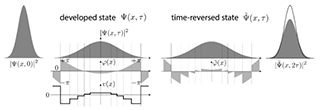
\includegraphics{imgs/fig-1.png}}}
    \caption{The \href{https://www.nature.com/articles/s41598-019-40765-6}{\textit{Time Reversal Procedure}}, using a \href{https://en.wikipedia.org/wiki/Quantum_computing}{\textit{Quantum Computer}}.}
    \label{fig}
  \end{figure}
\end{center}

\newpage

\subsection{Principles of \href{https://en.wikipedia.org/wiki/Quantum_computing}{Quantum Computing}}\label{AA}

The \href{https://en.wikipedia.org/wiki/Quantum_computing}{\textit{Quantum Computing}} promises to break many paradigms of \href{https://en.wikipedia.org/wiki/Von_Neumann_architecture}{\textit{Classical Computing}}, in which we can divide the problems into \href{http://www.cs.ucc.ie/~dgb/courses/toc/handout29.pdf}{\textit{"tractable problems"}}, that are problems that have reasonable, polynomial-time solutions and \href{http://www.cs.ucc.ie/~dgb/courses/toc/handout29.pdf}{\textit{"intractable problems"}}, that are problems that don't have it:

\begin{table}[!hp]
\centering
    \caption{Tractable and Intractable Problems in \href{https://en.wikipedia.org/wiki/Von_Neumann_architecture}{Classical Computing}}
    \begin{tabular}{ |p{2.2cm}|p{3cm}|p{2.2cm}| }
     \hline
     \begin{center}\textbf{\textit{Mathematical Notation}}\end{center} & \begin{center}\textbf{\textit{Complexity Time}}\end{center} & \begin{center}\textbf{\textit{Tractable/\\Intractable}}\end{center}\\
     \hline
     \hline
     \textbf{O(1)} & Constant & \textbf{Tractable} \\
     \hline
     $\bm{O(\log(n))}$ & Logarithmic & \textbf{Tractable} \\
     \hline
     \textbf{O(n)} & Linear & \textbf{Tractable} \\
     \hline
     $\bm{O(n\times\log(n))}$ & N-Log-N & \textbf{Tractable} \\
     \hline
     \textbf{O(n$^{2}$)} & Polynomial (Quadratic) & \textbf{Tractable} \\
     \hline
     \textbf{O(n$^{3}$)} & Polynomial (Cubic) & \textbf{Tractable} \\
     \hline
     \hline
     \textbf{O(k$^{n}$), e.g., O(2$^{n}$)} & Exponential & \textbf{Intractable} \\
     \hline
     \textbf{O(n!)} & Factorial & \textbf{Intractable} \\
     \hline
     \textbf{O(n$^{n}$)} & Super-Exponential & \textbf{Intractable} \\
     \hline
    \end{tabular}
\end{table}

\vspace{4pt}

The Moore's law predicted that computing should reach its limits by 2020s, as it becomes harder to produce processors and chips, in smaller dimensions and geometries:

\begin{center}
  \begin{figure}[htbp]
    \centerline{\href{https://en.wikipedia.org/wiki/Moore\%27s_law}{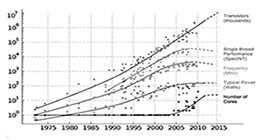
\includegraphics{imgs/fig-2.png}}}
    \caption{The prediction of the evolution of \href{https://en.wikipedia.org/wiki/Computing}{\textit{Computing}} by \href{https://en.wikipedia.org/wiki/Moore\%27s_law}{\textit{Moore's Law}}.}
    \label{fig}
  \end{figure}
\end{center}

However, it's already proved that it's possible (and feasible in the next 5 years) achieve the Quantum Computing that exceeds the reach of \href{https://en.wikipedia.org/wiki/Von_Neumann_architecture}{\textit{Classical Computers}}. This will mark the beginning of a new era of Quantum Science and Computing, at general.

\vspace{4pt}

All the elements that change the \href{https://en.wikipedia.org/wiki/Structure_and_Interpretation_of_Classical_Mechanics}{\textit{Classical Structures}} come from the changes that \href{https://en.wikipedia.org/wiki/Classical_physics}{\textit{Classical Physics}} has brought. \href{https://en.wikipedia.org/wiki/Physicist}{Physicists} like \href{https://en.wikipedia.org/wiki/Werner_Heisenberg}{\textit{Heisenberg}}, \href{https://en.wikipedia.org/wiki/Niels_Bohr}{\textit{Bohr}}, \href{https://en.wikipedia.org/wiki/Erwin_Schr\%C3\%B6dinger}{\textit{Schr\"odinger}}, and \href{https://en.wikipedia.org/wiki/Albert_Einstein}{\textit{Einstein}} studied these new foundations. Among them, it can be highlighted:

\vspace{6pt}

\begin{itemize}
  \item \textit{Quantum Overlap}:
    \begin{itemize}
        \item The \textit{Quantum Overlap} is a fundamental principle of \href{https://en.wikipedia.org/wiki/Quantum_mechanics}{\textit{Quantum Mechanics}} that states that a \href{https://en.wikipedia.org/wiki/Physical_system}{\textit{Physical System}} exists partially in all theoretically possible states simultaneously before being measured. But when measured or observed, the system is shown in a single state;
    \end{itemize}
  
  \newpage
  
  \item \href{https://en.wikipedia.org/wiki/Schr\%C3\%B6dinger\%27s_cat}{\textit{Schr\"odinger's Cat Experience}}:
    \begin{itemize}
        \item The \href{https://en.wikipedia.org/wiki/Schr\%C3\%B6dinger\%27s_cat}{\textit{Schr\"odinger's Cat}} is a mental experiment, often described as a paradox, developed by \href{https://en.wikipedia.org/wiki/Erwin_Schr\%C3\%B6dinger}{\textit{Erwin Schr\"odinger}}, in 1935. The experiment seeks to illustrate \href{https://en.wikipedia.org/wiki/Copenhagen_interpretation}{\textit{Copenhagen's Interpretation}} of \href{https://en.wikipedia.org/wiki/Quantum_mechanics}{\textit{Quantum Mechanics}} by imagining it applied to everyday objects. In the example, there's a cat enclosed in a box, so that it's not only alive or only dead, but "undead";
    \end{itemize}
  \begin{center}
      \begin{figure}[htbp]
        \centerline{\href{https://en.wikipedia.org/wiki/Schr\%C3\%B6dinger\%27s_cat}{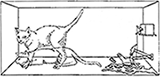
\includegraphics{imgs/fig-3.png}}}
        \caption{The \href{https://en.wikipedia.org/wiki/Schr\%C3\%B6dinger\%27s_cat}{\textit{Schr\"odinger's Cat Experience}}.}
        \label{fig}
      \end{figure}
  \end{center}
 
 \vspace{4pt}
 
  \item \href{https://en.wikipedia.org/wiki/Quantum_entanglement}{\textit{Quantum Entanglement} or \\\textit{"Ghostly Action at a Distance"}}:
   
    \begin{itemize}
        \item The \href{https://en.wikipedia.org/wiki/Quantum_entanglement}{\textit{Quantum Entanglement}} is a phenomenon of \href{https://en.wikipedia.org/wiki/Quantum_mechanics}{\textit{Quantum Mechanics}} that allows two or more objects to be somehow so connected that an object can't be correctly described without its counterpart be mentioned (even though the objects may be spatially separated by millions of \href{https://en.wikipedia.org/wiki/Light-year}{\textit{light years}}). This leads to very strong correlations between the observable \href{https://en.wikipedia.org/wiki/Physical_property}{\textit{physical properties}} of the various \href{https://en.wikipedia.org/wiki/Subatomic_particle}{\textit{subatomic particles}}. The \href{https://en.wikipedia.org/wiki/Quantum_entanglement}{\textit{Quantum Entanglement}} was called \href{https://en.wikipedia.org/wiki/Quantum_entanglement}{\textit{"Ghostly Action at a Distance"}} by \href{https://en.wikipedia.org/wiki/Albert_Einstein}{\textit{Albert Einstein}}, who believed it to be an impossible event under the laws of orthodox \href{https://en.wikipedia.org/wiki/Quantum_mechanics}{\textit{Quantum Mechanics}};
    \end{itemize}
    \begin{center}
      \begin{figure}[htbp]
        \centerline{\href{https://en.wikipedia.org/wiki/Quantum_entanglement}{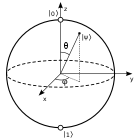
\includegraphics{imgs/fig-4.png}}}
        \caption{\href{https://en.wikipedia.org/wiki/Spontaneous_parametric_down-conversion}{Parametric Scattering}, using \href{https://en.wikipedia.org/wiki/Quantum_entanglement}{Quantum Entanglement}.}
        \label{fig}
      \end{figure}
  \end{center}
\end{itemize}

\begin{itemize}
  \item \href{https://en.wikipedia.org/wiki/Quantum_teleportation}{\textit{Quantum Teleportation}}:
    \begin{itemize}
        \item The \href{https://en.wikipedia.org/wiki/Quantum_teleportation}{\textit{Quantum Teleportation}} is a technology that allows teleportation of information, such as spin or polarization (there's no transport of energy or matter) by exclusively \href{https://en.wikipedia.org/wiki/Quantum}{\textit{Quantum}} means, which are independent of transmission media. The bandwidth for \href{https://en.wikipedia.org/wiki/Quantum_teleportation}{\textit{Quantum Teleportation}} doubled in 2015. It's a Chinese technique of transferring information about one particle so that another particle takes two instead of just one of the \href{https://en.wikipedia.org/wiki/Quantum}{\textit{Quantum}} properties of the initial particle;
    \end{itemize}

  \vspace{4pt}

  \item \href{https://en.wikipedia.org/wiki/Rutherford_scattering}{\textit{Rutherford Scattering}}:
    \begin{itemize}
        \item In \href{https://en.wikipedia.org/wiki/Physics}{Physics}, \href{https://en.wikipedia.org/wiki/Rutherford_scattering}{\textit{Rutherford's Dispersion}} is a phenomenon that was explained by \href{https://en.wikipedia.org/wiki/Ernest_Rutherford}{\textit{Ernest Rutherford}}, in 1909, and led to the development of the \href{https://en.wikipedia.org/wiki/Atomic_orbital}{\textit{orbital theory of the atom}}. It's now exploited by the \href{https://en.wikipedia.org/wiki/Rutherford_scattering}{\textit{Rutherford's Dispersion Spectrometry Material Analysis}} technique. The \href{https://en.wikipedia.org/wiki/Rutherford_scattering}{\textit{Rutherford's Dispersion}} is also sometimes referred to as \href{https://en.wikipedia.org/wiki/Rutherford_scattering}{\textit{Coulomb's Dispersion}} because it's based on \href{https://en.wikipedia.org/wiki/Electrostatics}{\textit{Electrostatic Forces}} (\href{https://en.wikipedia.org/wiki/Coulomb\%27s_law}{\textit{Coulomb}}). A similar process proved the core interior in the 1960s, called \href{https://arxiv.org/abs/1601.05453}{\textit{Inelastic Deep Dispersion}};
    \end{itemize}
    
  \vspace{4pt}
    
  \item \textit{Existence of Multiverse}:
    \begin{itemize}
        \item The \href{https://en.wikipedia.org/wiki/Many-worlds_interpretation}{\textit{Quantum Multiverse}} (also known as \href{https://en.wikipedia.org/wiki/Many-worlds_interpretation}{\textit{Multiverse Theory}} or \href{https://en.wikipedia.org/wiki/Many-worlds_interpretation}{\textit{Many-worlds' Interpretation}}) is an interpretation of \href{https://en.wikipedia.org/wiki/Quantum_mechanics}{\textit{Quantum Mechanics}} that asserts the objective reality of the universal wave-function and denies the actuality of wave-function collapse. The existence of the other worlds makes it possible to remove randomness and action at a distance from \href{https://en.wikipedia.org/wiki/Quantum_theory}{\textit{Quantum Theory}} and thus from all \href{https://en.wikipedia.org/wiki/Physics}{\textit{Physics}}. The \href{https://en.wikipedia.org/wiki/Many-worlds_interpretation}{\textit{Quantum Multiverse}} implies that all possible alternate histories and futures are real, each representing an actual "world" (or "universe");
    \end{itemize}
\end{itemize}

\vspace{6pt}

And it was thanks to these principles that the development of \href{https://en.wikipedia.org/wiki/Quantum_computing}{\textit{Quantum Computing}} was possible.

\vspace{6pt}

\section{Learning about \href{https://en.wikipedia.org/wiki/Quantum}{Quantum}}

\subsection{Understanding the \href{https://en.wikipedia.org/wiki/Quantum_computing}{\textit{Quantum Computing}}}\label{AA}

The \href{https://en.wikipedia.org/wiki/Quantum_mechanics}{\textit{Quantum Mechanics}} is considered to be the most successful \href{https://en.wikipedia.org/wiki/Theoretical_physics}{\textit{Physical Theory}}. For from its creation to the present day, it has been applied in diverse branches, from \href{https://en.wikipedia.org/wiki/Particle_physics}{\textit{Particle Physics}}, \href{https://en.wikipedia.org/wiki/Atomic_and_molecular_astrophysics}{\textit{Atomic and Molecular Astrophysics}}, and \href{https://en.wikipedia.org/wiki/Condensed_matter_physics}{\textit{Condensed Matter Physics}}.

\vspace{4pt}

In \href{https://en.wikipedia.org/wiki/Quantum_computing}{\textit{Quantum Computing}}, the basic information unit's the \href{https://en.wikipedia.org/wiki/Qubit}{\textit{Quantum Bit}} or \href{https://en.wikipedia.org/wiki/Qubit}{\textit{Qubit}}. The fact that \href{https://en.wikipedia.org/wiki/Quantum_computing}{\textit{Quantum Computing}} it's so powerful lies in the fact that in addition to assuming zero ('$\textit{\textbf{0}}$') and one ('$\textit{\textbf{1}}$'), as in \href{https://en.wikipedia.org/wiki/Von_Neumann_architecture}{\textit{Classical Computing}}'s memory (following the \href{https://en.wikipedia.org/wiki/Von_Neumann_architecture}{\textit{Von Neumann's Architecture}}) made up of \href{https://en.wikipedia.org/wiki/Bit}{\textit{bits}}, it can assume both zero ('$\textit{\textbf{0}}$') and one ('$\textit{\textbf{1}}$') states at the same time by \href{https://en.wikipedia.org/wiki/Quantum_superposition}{\textit{Quantum Superposition}} of those 2 \href{https://en.wikipedia.org/wiki/Qubit}{\textit{qubit}} states.

\vspace{4pt}

A pair of \href{https://en.wikipedia.org/wiki/Qubit}{\textit{qubits}} can be in any \href{https://en.wikipedia.org/wiki/Quantum_superposition}{\textit{Quantum Superposition}} of 4 states, and 3 \href{https://en.wikipedia.org/wiki/Qubit}{\textit{qubits}} in any superposition of 8 states. In general, a \href{https://en.wikipedia.org/wiki/Quantum_computing}{\textit{Quantum Computer}} with \textit{n \href{https://en.wikipedia.org/wiki/Qubit}{qubits}} can be in any superposition of up to 2\textsuperscript{n} different states (in comparison to a normal computer that can only be in one of these 2\textsuperscript{n} states at any one time).

\vspace{4pt}

It's hard to assume the two different states at the same time, but \href{https://en.wikipedia.org/wiki/Schr\%C3\%B6dinger\%27s_cat}{\textit{Schr\"odinger's Cat's Mental Experience}} can give an intuitive sense to the situation. And it's thanks to this property of the \href{https://en.wikipedia.org/wiki/Quantum_superposition}{\textit{Quantum Superposition}} of states that motivated the studies in \textit{Quantum Computing}. If in \href{https://en.wikipedia.org/wiki/Von_Neumann_architecture}{\textit{Classical Computing}}, the processing is sequential, in the \href{https://en.wikipedia.org/wiki/Quantum_computing}{\textit{Quantum Computing}}, the processing is simultaneous.

\vspace{4pt}

The \href{https://en.wikipedia.org/wiki/Qubit}{\textit{qubit}} is described by a states' vector in a two-level \href{https://en.wikipedia.org/wiki/Quantum_system}{\textit{Quantum System}}, which is equivalent to a two-dimensional space's vector over complex numbers. The \href{https://en.wikipedia.org/wiki/Bra\%E2\%80\%93ket_notation}{\textit{bra-ket's notation}} is used to represent them:

\vspace{4pt}

\begin{itemize}
    \item 
    \begin{center}
        $\mid$\textbf{0}$\rangle$ = ${
            \begin{bmatrix}
                \textbf{1}\\
                \textbf{0}
            \end{bmatrix}}$ 
        or even, 
        $\mid$\textbf{1}$\rangle$ = ${
            \begin{bmatrix}
                \textbf{0}\\
                \textbf{1}
            \end{bmatrix}}$ 
    \end{center}
\end{itemize}

\vspace{4pt}

Thus, the state of a \href{https://en.wikipedia.org/wiki/Qubit}{\textit{qubit}} can be represented by:

\vspace{4pt}

\begin{itemize}
    \item 
    \begin{center}
        $\mid$$\psi$$\rangle$ = $\alpha$$\mid$\textbf{0}$\rangle$ + $\beta$$\mid$\textbf{1}$\rangle$
    \end{center}
\end{itemize}

\vspace{4pt}

The set \{$\mid$\textbf{0}$\rangle$, $\mid$\textbf{1}$\rangle$\} forms a two-dimensional \href{https://en.wikipedia.org/wiki/Hilbert_space}{\textit{Hilbert's Space}} called the \href{https://en.wikipedia.org/wiki/Controlled_NOT_gate#Behaviour_in_the_Hadamard_transformed_basis}{\textit{Computational or Hadamard Transformed Basis}}.

\begin{figure}[htbp]
\centerline{\href{https://en.wikipedia.org/wiki/Qubit}{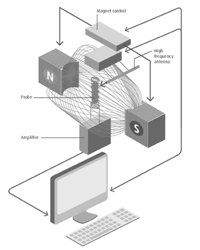
\includegraphics{imgs/fig-5.png}}}
\caption{\href{https://en.wikipedia.org/wiki/Bloch_sphere}{\textit{Bloch Sphere representation}} of a \href{https://en.wikipedia.org/wiki/Qubit}{\textit{Qubit}}.}
\label{fig}
\end{figure}


\vspace{4pt}

For the manipulation of \href{https://en.wikipedia.org/wiki/Quantum_state}{\textit{Quantum States}}, some kind of \href{https://en.wikipedia.org/wiki/Electromagnetic_radiation}{\textit{Optical Techniques}, \textit{i.e.}, \textit{Electromagnetic Radiation}}, are used. These devices constitute \href{https://en.wikipedia.org/wiki/Quantum_logic_gate}{\textit{Quantum Logic Gates}}. A \href{https://en.wikipedia.org/wiki/Quantum_computing}{\textit{Quantum Computer}} operates on its \href{https://en.wikipedia.org/wiki/Qubit}{\textit{qubits}} using this \href{https://en.wikipedia.org/wiki/Quantum_logic_gate}{\textit{Quantum Logic Gates}} and measurement (which also alters the observed state). This manipulation can be performed using \href{https://en.wikipedia.org/wiki/Atom}{\textit{atoms}} that can be excited or not, or even, the both, at the same time.

\vspace{4pt}

Another device used is the manipulation of \href{https://en.wikipedia.org/wiki/Photon}{\textit{photons}}. The advantage of using them lies in the fact that these \href{https://en.wikipedia.org/wiki/Photon}{\textit{photons}} can constitute highly stable carriers of \href{https://en.wikipedia.org/wiki/Quantum_information}{\textit{Quantum Information}}.

\vspace{4pt}

However, \href{https://en.wikipedia.org/wiki/Photon}{\textit{photons}} don't interact directly with each other, requiring the use of an \href{https://en.wikipedia.org/wiki/Atom}{\textit{atom}} as a mediator, which introduces additional noise and complications in the experiments. In this case, a \href{https://en.wikipedia.org/wiki/Photon}{\textit{photon}} interacts with an \href{https://en.wikipedia.org/wiki/Atom}{\textit{atom}} which in turn interacts with the second \href{https://en.wikipedia.org/wiki/Photon}{\textit{photon}}, leading to the complete interaction between the two \href{https://en.wikipedia.org/wiki/Photon}{\textit{photons}}.

\vspace{4pt}

 A \href{https://en.wikipedia.org/wiki/Quantum_algorithm}{\textit{Quantum Algorithm}} is composed of a fixed sequence of \href{https://en.wikipedia.org/wiki/Quantum_logic_gate}{\textit{Quantum Logic Gates}} and a problem is encoded by setting the initial values of the \href{https://en.wikipedia.org/wiki/Qubit}{\textit{qubits}}, similar to how a \href{https://en.wikipedia.org/wiki/Von_Neumann_architecture}{\textit{Classical Computer}} works.
 
 \vspace{4pt}
 
 The calculation usually ends with a measurement, collapsing the system of \href{https://en.wikipedia.org/wiki/Qubit}{\textit{qubits}} into one of the 2\textsuperscript{n} \href{https://en.wikipedia.org/wiki/Quantum_state#Pure_states}{\textit{eigenstates (or pure states)}}, where each \href{https://en.wikipedia.org/wiki/Qubit}{\textit{qubit}} is zero ('$\textit{\textbf{0}}$') or one ('$\textit{\textbf{1}}$'), decomposing into a classical state. The outcome can, therefore, be at most \textit{n} classical \href{https://en.wikipedia.org/wiki/Bit}{\textit{bits}} of information. If the algorithm didn't end with a measurement, the result is an unobserved \href{https://en.wikipedia.org/wiki/Quantum_state}{\textit{Quantum State}} (such unobserved states may be sent to other computers as part of \textit{Distributed Quantum Algorithms}).

\newpage

The \textit{Quantum Algorithms} are often probabilistic, in that they provide the correct solution only with a certain known probability. Note that the term \href{https://en.wikipedia.org/wiki/Non-deterministic_Turing_machine}{\textit{non-deterministic computing}} mustn't be used in that case to mean probabilistic (\href{https://en.wikipedia.org/wiki/Computing}{\textit{computing}}) because the term non-deterministic has a different meaning in \href{https://en.wikipedia.org/wiki/Computer_science}{\textit{Computer Science}} and \href{https://en.wikipedia.org/wiki/Informatics}{\textit{Informatics}}.

\vspace{4pt}

In order to store the \href{https://en.wikipedia.org/wiki/Qubit}{\textit{qubits}}, \href{https://en.wikipedia.org/wiki/Ion_trap}{\textit{ion's traps}} are used, in which a small number of charged \href{https://en.wikipedia.org/wiki/Atom}{\textit{atoms}} are trapped, and also, \href{https://en.wikipedia.org/wiki/Magnetic_trap_(atoms)}{\textit{neutral ion's traps}} to trap uncharged \href{https://en.wikipedia.org/wiki/Atom}{\textit{atoms}}.

\vspace{4pt}

In this scheme, the \href{https://en.wikipedia.org/wiki/Photon}{\textit{photons}} are used to manipulate the information contained in the \href{https://en.wikipedia.org/wiki/Atom}{\textit{atoms}}, in this way they constitute a type of \href{https://en.wikipedia.org/wiki/Quantum_logic_gate}{\textit{Quantum Logic Gates}} that applies appropriate \textit{pulses of \href{https://en.wikipedia.org/wiki/Electromagnetic_radiation}{electromagnetic radiation}} so that the \href{https://en.wikipedia.org/wiki/Atom}{\textit{atoms}} in the neighborhood can interact with each other like via, per example, \href{https://en.wikipedia.org/wiki/Intermolecular_force}{\textit{dipole forces}}.

\vspace{4pt}

Another class of \href{https://en.wikipedia.org/wiki/Quantum_information_science}{\textit{Quantum Information Processing}} is based on \href{https://en.wikipedia.org/wiki/Nuclear_magnetic_resonance}{\textit{Nuclear Magnetic Resonance}} (\href{https://en.wikipedia.org/wiki/Nuclear_magnetic_resonance}{\textit{NMR}}). In this case, the \href{https://en.wikipedia.org/wiki/Quantum_information}{\textit{Quantum Information}} is stored in the \href{https://en.wikipedia.org/wiki/Spin_(physics)}{\textit{nuclear spins}} of the \href{https://en.wikipedia.org/wiki/Atom}{\textit{atoms}} in \href{https://en.wikipedia.org/wiki/Molecule}{\textit{molecules}} and the \href{https://en.wikipedia.org/wiki/Quantum_logic_gate}{\textit{Quantum Logical Gates}} manipulate that information using the \href{https://en.wikipedia.org/wiki/Electromagnetic_radiation}{\textit{electromagnetic radiation}}.

\vspace{4pt}

This is an example of an implementation of \href{https://en.wikipedia.org/wiki/Qubit}{\textit{qubits}} in a \href{https://en.wikipedia.org/wiki/Quantum_computing}{\textit{Quantum Computer}}, where could start with the use of \href{https://en.wikipedia.org/wiki/Particle}{\textit{particles}} (\href{https://en.wikipedia.org/wiki/Electron}{\textit{electrons}}) with two \href{https://en.wikipedia.org/wiki/Spin_State}{\textit{spin states}}: \textit{"down"} and \textit{"up"}, as also, the both at the same time (typically written \textbf{$\mid\downarrow\rangle$} and \textbf{$\mid\uparrow\rangle$}, or \textbf{$\mid$0$\rangle$} and \textbf{$\mid$1$\rangle$}). This is true because any such system can be mapped onto an effective \href{https://en.wikipedia.org/wiki/Spin-\%C2\%BD}{\textit{spin-$\frac{1}{2}$ system}}.

\vspace{4pt}

The \href{https://en.wikipedia.org/wiki/Nuclear_magnetic_moment}{\textit{nuclear magnetic moments}} make a \href{https://en.wikipedia.org/wiki/Precession}{\textit{natural precession movement}} in the presence of \href{https://en.wikipedia.org/wiki/Magnetic_field}{\textit{magnetic fields}}. The \href{https://en.wikipedia.org/wiki/Quantum_state}{\textit{Quantum States}} of the cores can be manipulated by irradiating the cores with \href{https://en.wikipedia.org/wiki/Radio_frequency}{\textit{radio frequency pulses}} tuned to the \href{https://en.wikipedia.org/wiki/Precession}{\textit{precession frequency}} of these.

\vspace{4pt}

In a given compound made up of \href{https://en.wikipedia.org/wiki/Atom}{\textit{atoms}}, can be measured the resonances of the cores of some of them, without altering them, using \href{https://en.wikipedia.org/wiki/Nuclear_magnetic_resonance}{\textit{Nuclear Magnetic Resonance}} (\href{https://en.wikipedia.org/wiki/Nuclear_magnetic_resonance}{\textit{NMR}}). It's sensitive to the interactions of the \href{https://en.wikipedia.org/wiki/Nuclear_magnetic_moment}{\textit{nuclear moments}} exposed to the \href{https://en.wikipedia.org/wiki/Electric_field}{\textit{local electric}} and \href{https://en.wikipedia.org/wiki/Magnetic_field}{\textit{magnetic fields}}, called \href{https://en.wikipedia.org/wiki/Hyperfine_structure}{\textit{hyper-fines}}. Each type of \href{https://en.wikipedia.org/wiki/Spin_states_(d_electrons)}{\textit{spin}} has an \href{https://en.wikipedia.org/wiki/Angular_velocity}{\textit{angular velocity}} that depends on the applied field and the exchange interaction between them.

\begin{figure}[htbp]
\centerline{\href{https://en.wikipedia.org/wiki/Nuclear_magnetic_resonance}{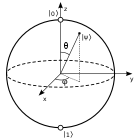
\includegraphics{imgs/fig-6.png}}}
\caption{\href{https://en.wikipedia.org/wiki/Nuclear_magnetic_resonance}{\textit{Nuclear Magnetic Resonance}} (\href{https://en.wikipedia.org/wiki/Nuclear_magnetic_resonance}{\textit{NMR}}).}
\label{fig}
\end{figure}

\newpage

Just as in \href{https://en.wikipedia.org/wiki/Von_Neumann_architecture}{\textit{Classical Computing}}, in \href{https://en.wikipedia.org/wiki/Quantum_computing}{\textit{Quantum Computing}} are used \href{https://en.wikipedia.org/wiki/Circuit}{\textit{Circuits}}, but these \href{https://en.wikipedia.org/wiki/Circuit}{\textit{Circuits}} are \href{https://en.wikipedia.org/wiki/Quantum}{\textit{Quantum}}.

\vspace{4pt}

So, \textit{logical operations} or even \textit{algorithms}, can be described by a \href{https://en.wikipedia.org/wiki/Quantum_circuit}{\textit{Quantum Circuit}}. In these \href{https://en.wikipedia.org/wiki/Circuit}{\textit{Circuits}}, can be used the \href{https://en.wikipedia.org/wiki/Logic_gate}{\textit{Logic Gates}} used in \href{https://en.wikipedia.org/wiki/Von_Neumann_architecture}{\textit{Classical Computing}}, but it's possible to use others that may allow, per example, the construction of a \textit{possible circuit for the teleportation of data}.

\vspace{4pt}

However, in the same way that, the property of \href{https://en.wikipedia.org/wiki/Quantum_superposition}{\textit{Superposition of States}} allows the creation of the \href{https://en.wikipedia.org/wiki/Quantum_computing}{\textit{Quantum Computer}}, it's this same property that makes it impossible to create them.

\vspace{4pt}

The difficulties of creating a \href{https://en.wikipedia.org/wiki/Quantum_computing}{\textit{Quantum Computer}} lie in the fact that the computational processes happen to be in the \href{https://en.wikipedia.org/wiki/Atom}{\textit{atomic universe}}, that lacks of technologies of manipulation still.

\vspace{4pt}

One of the main problems, for example, is the high error rate caused by the environment due to the extreme sensitivity of the technology. The \href{https://en.wikipedia.org/wiki/Quantum_superposition}{\textit{Superposition of States}} is very sensitive to any \textit{electromagnetic micro-disturbance} that can alter the state of the \href{https://en.wikipedia.org/wiki/Qubit}{\textit{qubit}} causing the information contained in it to be lost.

\vspace{4pt}

Another important fact in question is the \textit{overheating of the machines}. For that reason it's almost mandatory use this kind of systems cooled with temperatures close to \href{https://en.wikipedia.org/wiki/Absolute_zero}{\textit{"absolute zero"}}.

\vspace{4pt}

\begin{center}
  \begin{figure}[htbp]
    \centerline{\href{https://www.research.ibm.com/ibm-q/}{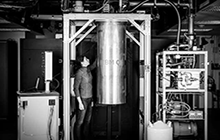
\includegraphics{imgs/fig-7.png}}}
    \caption{The \href{https://www.research.ibm.com/ibm-q/}{\textit{IBM Q's Quantum Computer}}.}
    \label{fig}
  \end{figure}
\end{center}

\subsection{Current research in \href{https://en.wikipedia.org/wiki/Quantum_computing}{\textit{Quantum Computing}} Worldwide and in Portugal}\label{AA}

\vspace{4pt}

There's no such thing as a fully functioning \href{https://en.wikipedia.org/wiki/Quantum_computing}{\textit{Quantum Computer}} today. However, companies such as \href{https://en.wikipedia.org/wiki/D-Wave_Systems}{\textit{D-Wave System}}, \href{https://en.wikipedia.org/wiki/Google}{\textit{Google}} and \href{https://en.wikipedia.org/wiki/IBM}{\textit{IBM}}, among others, have made promises, which if fulfilled, will announce a new horizon for the reality and market of home, scientific and corporate computers.

\vspace{4pt}

Many \href{https://en.wikipedia.org/wiki/Quantum_computing}{\textit{Quantum Computer Prototypes}} have already been tested in laboratories worldwide, but their large-scale development may still be far away and dependent on much research and investment.

\vspace{4pt}

In 2018, the \href{https://www.it.pt/}{\textit{Physics of Information and Quantum Technologies Group of the Instituto de Telecomunica\c{c}\"oes}}, headquartered at \href{https://tecnico.ulisboa.pt/}{\textit{Instituto Superior T\'ecnico}}, won a total funding of \euro\hspace{0.05mm} 13 million supported by \href{https://qt.eu/}{\textit{Quantum Flagship}} for 2 research projects called \href{http://quantum-internet.team/}{\textit{"Quantum Internet Alliance"}} and \href{https://ec.europa.eu/digital-single-market/en/content/qmics-quantum-microwave-communication-and-sensing}{\textit{"Quantum Microwave Communication and Sensing"}}.

\newpage

The \href{http://quantum-internet.team/}{\textit{"Quantum Internet Alliance"}} intends to build in the next three years, the first prototype of the future \href{https://en.wikipedia.org/wiki/Quantum_network#Quantum_internet}{\textit{Quantum Internet}}, a network that could allow private long distance communications, as well as \href{https://en.wikipedia.org/wiki/Quantum_network}{\textit{Networking Quantum Computers}} and \href{https://en.wikipedia.org/wiki/Quantum_sensor}{\textit{Quantum Sensor Systems}}.

\vspace{4pt}

In this challenge, the researchers of the \href{https://tecnico.ulisboa.pt/}{\textit{Instituto Superior T\'ecnico}} have the partnership of researchers from the \href{https://www.tudelft.nl/}{\textit{Technical University of Delft}}, the \href{https://www.mpq.mpg.de/}{\textit{Max-Planck-Institute for Quantum Optics}}, the \href{https://www.nbi.ku.dk/}{\textit{Niels Bohr Institute}} and the \href{https://www.oeaw.ac.at/}{\textit{Austrian Academy of Science}}, among others.

\vspace{4pt}

For the first time, will be tried to be built a \href{https://en.wikipedia.org/wiki/Quantum_network}{\textit{Quantum Network}} that will serve any \href{https://en.wikipedia.org/wiki/Quantum}{\textit{Quantum}} \textit{Application}: \href{https://en.wikipedia.org/wiki/Secure_communication}{\textit{Secure Communications}}, \href{https://en.wikipedia.org/wiki/Distributed_computing}{\textit{Distributed Computing}}, \href{https://en.wikipedia.org/wiki/Quantum_sensor}{\textit{Quantum Sensor Networks}}, etc. It's a \href{https://en.wikipedia.org/wiki/Quantum_network#Quantum_internet}{\textit{Quantum Internet}}, never tried before.

\vspace{4pt}

The \href{https://ec.europa.eu/digital-single-market/en/content/qmics-quantum-microwave-communication-and-sensing}{\textit{"Quantum Microwave Communication and Sensing"}}, with the involvement of the \href{https://www.wmi.badw.de/}{\textit{Walther-Meissner-Institut}}, the \href{http://www.ens-lyon.fr/}{\textit{École Normale Supérieure de Lyon}} and \href{https://www.oxinst.com/}{\textit{Oxford Instruments}}, among others, is a fundamental research project, which is the superconductor of a program that operates at \href{https://en.wikipedia.org/wiki/Absolute_zero}{\textit{"absolute zero"}} temperature to generate interwoven \href{https://en.wikipedia.org/wiki/Microwave}{\textit{microwaves}}.

\vspace{4pt}

The goal it's to build a system without the knowledge or interaction with itself, using \href{https://en.wikipedia.org/wiki/Quantum_entanglement}{\textit{Quantum Interlacing}}. This research can leads it to have important applications such as, for example, \href{https://en.wikipedia.org/wiki/Quantum_radar}{\textit{Quantum Radars}}, much more sensitive than the current radars.

\vspace{4pt}

Recently, the \href{https://sigarra.up.pt/fcup/pt/web_page.inicial}{\textit{Faculty of Sciences of University of Porto}} also already adopted a course of \href{https://en.wikipedia.org/wiki/Quantum_computing}{\textit{Quantum Computing}} in their \textit{Informatics' PhD} degree.

\vspace{4pt}

Also in 2018, the \href{http://www.quantalab.org/}{\textit{QuantaLab}}, led by the \href{https://www.uminho.pt/PT}{\textit{University of Minho}}, and composed also by, \href{https://www.inesctec.pt/en}{\textit{Instituto de Engenharia de Sistemas e Computadores, Tecnologia e Ci\^encia (INESC TEC)}} and the \href{https://www.ceiia.com/}{\textit{Centro de Excel\^encia para a Inova\c{c}\"ao da Ind\'ustria Autom\'ovel (CEiiA)}}, started to be part of the largest international \textit{Quantum Computing Network}, entering into the \textit{IBM Q Network}, as an academic partner.

\vspace{4pt}

In 2019, the \href{https://www.fct.pt/}{\textit{Funda\c{c}\~{a}o para a Ci\^{e}ncia e Tecnologia}}, launched an initiative called \textit{Quantum Portugal} aiming to attract new researchers for \href{https://en.wikipedia.org/wiki/Quantum_computing}{\textit{Quantum Computing}}, with the funding of \textit{PhD} scholarships.

\vspace{4pt}

The goal of this initiative it's, essentially, the \textit{Creation of New \href{https://en.wikipedia.org/wiki/Medication}{Medicines} and \href{https://en.wikipedia.org/wiki/Materials_science}{Materials}, \href{https://en.wikipedia.org/wiki/Financial_risk_management}{Financial Risk Analysis}, \href{https://en.wikipedia.org/wiki/Inventory}{Inventory Management}, \href{https://en.wikipedia.org/wiki/Facial_recognition_system}{Facial Recognition}, \href{https://en.wikipedia.org/wiki/Artificial_intelligence}{Artificial Intelligence}, as also, Simulation and Testing of, \href{https://en.wikipedia.org/wiki/Condensed_matter_physics}{Condensed Matter Physics}, \href{https://en.wikipedia.org/wiki/Materials_science}{Materials Science}, \href{https://en.wikipedia.org/wiki/Process_optimization}{Process Optimization} and \href{https://en.wikipedia.org/wiki/Computer_security}{Cybersecurity}}.

\vspace{4pt}

This contest will be managed by the \href{https://inl.int/}{\textit{Laborat\'orio Ib\'erico Internacional de Nanotecnologia}} and will make their infrastructures available, as a host institution for \textit{PhD} students from universities over all Portugal.

\vspace{4pt}

Also, in 2019, \href{https://noticias.up.pt/estudante-feup-vence-premio-internacional-em-computacao-quantica/}{\textit{Miguel Ramalho}}, of \href{https://sigarra.up.pt/feup/pt/web_page.inicial}{\textit{Faculty of Engineering of University of Porto}} won the \href{https://www.ibm.com/blogs/research/2019/01/ibmq-teach-quantum-winners/}{\textit{"IBM Q Teach Me Quantum"}}, initiative that challenges the creation of a course in \href{https://en.wikipedia.org/wiki/Quantum_computing}{\textit{Quantum Computing}} that integrates the tools developed by \href{https://en.wikipedia.org/wiki/IBM}{\textit{IBM}} in recent years.

\newpage

\subsection{Understanding (better) the \href{https://en.wikipedia.org/wiki/Qubit}{Quantum Bit (or Qubit)}}\label{AA}

\vspace{4pt}

Since, a \href{https://en.wikipedia.org/wiki/Quantum_state}{\textit{Quantum State}} can represent 2 states, at the same time, it's reasonable to think that a \href{https://en.wikipedia.org/wiki/Qubit}{\textit{qubit}} also could represent 2 \href{https://en.wikipedia.org/wiki/Bit}{\textit{bits}}, at once. So, \textit{n \href{https://en.wikipedia.org/wiki/Qubit}{qubits}} can be represented as 2\textsuperscript{n} \href{https://en.wikipedia.org/wiki/Bit}{\textit{bits}}.

\vspace{4pt}

For comprehension of the \textit{computational power} that will be analysed, consider some statistics from \href{http://www.statsoft.com/Products/STATISTICA-Features}{\textit{StatSoft's Statistica}}:

\begin{figure}[htbp]
\centerline{\href{https://www.statista.com/statistics/795748/worldwide-seagate-average-hard-disk-drive-capacity/}{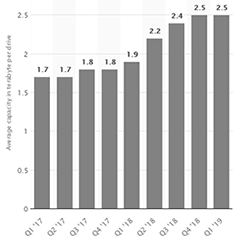
\includegraphics{imgs/fig-8.png}}}
\caption{Average capacity of \href{https://www.seagate.com/}{\textit{Seagate}} \href{https://en.wikipedia.org/wiki/Hard_disk_drive}{\textit{Hard Disk Drives}} worldwide from 2017 to 2019, by quarter (in \textit{terabyte} per drive).}
\label{fig}
\end{figure}

This statistics revealed that the average capacity of \href{https://www.seagate.com/}{\textit{Seagate}}'s \href{https://en.wikipedia.org/wiki/Hard_disk_drive}{\textit{Hard Disk Drives}}, at the first quarter of 2019 year was approximately 2.5 \textit{terabytes} per drive.

\vspace{4pt}

The following table shows the increase of the data that can be processed and kept by \href{https://en.wikipedia.org/wiki/Qubit}{\textit{qubits}}, in comparison to \href{https://en.wikipedia.org/wiki/Bit}{\textit{bits}}:

\begin{table}[!hp]
\centering
    \caption{Comparison of Quantum Values (SuperDense Coding)}
    \begin{tabular}{ |p{1.6cm}|p{6.2cm}| }
     \hline
     \multicolumn{2}{|c|}{\textbf{\textit{Qubits (Quantum Bits)} vs. \textit{Bits}}} \\
     \hline
     \hline
     \textbf{\# Qubits} & \textbf{\# Bits}\\
     \hline
     \hline
     \textbf{1 qubit} & 2 bits \\
     \hline
     \textbf{2 qubits} & 4 bits \\
     \hline
     \textbf{3 qubits} & 8 bits = 1 B \\
     \hline
     \textbf{4 qubits} & 16 bits \\
     \hline
     \textbf{5 qubits} & 32 bits \\
     \hline
     \textbf{6 qubits} & 64 bits \\
     \hline
     \textbf{7 qubits} & 128 bits \\
     \hline
     \textbf{8 qubits} & 256 bits \\
     \hline
     \textbf{9 qubits} & 512 bits \\
     \hline
     \textbf{10 qubits} & 1,024 bits \\
     \hline
     \textbf{13 qubits} & 8,192 bits $\approx$ 1 KB \\
     \hline
     \textbf{23 qubits} & 8,388,608 bits $\approx$ 1 MB \\
     \hline
     \textbf{33 qubits} & 8,589,934,592 bits $\approx$ 1 GB \\
     \hline
     \textbf{43 qubits} & 8,796,093,022,208 bits $\approx$ 1 TB \\
     \hline
     \textbf{44 qubits} & 17,592,186,044,416 bits $\approx$ 2 TBs \\
     \hline
     \textbf{45 qubits} & 35,184,372,088,832 bits $\approx$ 4 TBs \\
     \hline
     \textbf{50 qubits} & 1,125,899,906,842,624 bits $\approx$ 128 TBs \\
     \hline
     \hline
     \textbf{72 qubits} & 4,722,366,482,869,645,213,696 bits $\approx$ \\ & 
     $\approx$ 536,870,912 TBs $\approx$ 512 EBs $\approx$ 0.5 ZBs \\
     \hline
     \textbf{2,000 qubits} & $\approx$ 1.15$\times$10$^{602}$ ‬bits $\approx$ 1.44$\times$10$^{586}$ TBs $\approx$ \\ & $\approx$ 1.44$\times$10$^{579}$ EBs $\approx$ 1.44$\times$10$^{576}$ ZBs $\approx$ \\ & $\approx$ 1.44$\times$10$^{573}$ YBs $\approx$ 144,000,000,000$\times$10$^{562}$ YBs\\
     \hline
     \hline
     \textbf{n qubits} & 2\textsuperscript{n} bits \\
     \hline
    \end{tabular}
\end{table}

\newpage

Following the statistics from \href{http://www.statsoft.com/Products/STATISTICA-Features}{\textit{StatSoft's Statistica}}, at average, each \textit{classic computer} would have a \href{https://en.wikipedia.org/wiki/Hard_disk_drive}{\textit{HDD}} of 2.5 \textit{terabytes} of capacity. A \href{https://en.wikipedia.org/wiki/Quantum}{\textit{Quantum}} \textit{chip} of 72 \href{https://en.wikipedia.org/wiki/Qubit}{\textit{qubits}}, such as \href{https://ai.googleblog.com/2018/03/a-preview-of-bristlecone-googles-new.html}{\textit{Bristlecone}}, would be 214,748,364$\times$ more powerful than each one of them.

\vspace{4pt}

In another perspective, could be thought that was predicted that, the volume of the entire \href{https://en.wikipedia.org/wiki/Internet}{\textit{Internet}} in the world, in 2016, would be 1.3 \textit{zettabytes}. The same \href{https://en.wikipedia.org/wiki/Quantum}{\textit{Quantum}} \textit{chip} of 72 \href{https://en.wikipedia.org/wiki/Qubit}{\textit{qubits}} would represent almost half of this huge amount of data.

\vspace{4pt}

So, it's unthinkable the computing power that a \href{https://en.wikipedia.org/wiki/Quantum_computing}{\textit{Quantum Computer}}, as \href{https://en.wikipedia.org/wiki/D-Wave_Systems#D-Wave_2X_and_D-Wave_2000Q}{\textit{D-Wave's 2000Q}} could have. A huge quantity of the problems that \textit{classic computers} couldn't resolve at a reasonable time, would be resolved easily, at polynomial-time.

\vspace{6pt}

\section{\href{https://en.wikipedia.org/wiki/Quantum_computing}{Quantum Computing} in \href{https://en.wikipedia.org/wiki/Internet_security}{Security of Internet and World Wide Web (WWW)}}

\vspace{4pt}

\subsection{How can \href{https://en.wikipedia.org/wiki/Quantum_computing}{Quantum Computing} impact \href{https://en.wikipedia.org/wiki/Internet_security}{Internet's Security}?}\label{AA}

\vspace{4pt}

The main limitation of \href{https://en.wikipedia.org/wiki/Symmetric-key_algorithm}{\textit{Symmetric Cryptography}} is the keys' distribution, since after their generation they've to be sent to the endpoints. Although, the message with the key can also be intercepted and would need a secure means to be sent.

\vspace{4pt}

In the 1970s, with the development of systems that used \href{https://en.wikipedia.org/wiki/Public-key_cryptography}{\textit{Asymmetric Cryptography}}, the problem became semi-resolved, since it would no longer be necessary to distribute the keys.

\vspace{4pt}

Currently, the most common \href{https://en.wikipedia.org/wiki/Public-key_cryptography}{\textit{Public Key}} \href{https://en.wikipedia.org/wiki/Cryptosystem}{\textit{Cryptosystem}}, the \href{https://en.wikipedia.org/wiki/RSA_(cryptosystem)}{\textit{Rivest-Shamir-Adleman (RSA)}}, is based on numbers' factorization, that only offer some safety due to the current computational limitation, such as the difficulty of factorization of large prime numbers, discrete logarithms, among others.

\vspace{4pt}

Improved approaches to factoring large numbers, such as \href{https://en.wikipedia.org/wiki/Shor\%27s_algorithm}{\textit{Shor's Algorithm}} running on a sufficiently powerful \href{https://en.wikipedia.org/wiki/Quantum_computing}{\textit{Quantum Computer}}, will improve the likelihood of breaking an algorithm of \href{https://en.wikipedia.org/wiki/Public-key_cryptography}{\textit{Public-Key Encryption}}.

\vspace{4pt}

The \href{https://en.wikipedia.org/wiki/Quantum_computing}{\textit{Quantum Computing}} offers the potential for breaking the \href{https://en.wikipedia.org/wiki/Public-key_cryptography}{\textit{Public-Key Encryption}} standards that protect all of the data, safely stored, shared and used, through the \href{https://en.wikipedia.org/wiki/Internet}{\textit{Internet}}.

\vspace{4pt}

The following table provides which of these encryption algorithms are breakable using current \href{https://en.wikipedia.org/wiki/Quantum_computing}{\textit{Quantum Computing}}:

\begin{table}[!hp]
\centering
    \caption{Encryption Algorithms breakable from Quantum Computing}
    \begin{tabular}{ |p{4cm}|p{2.5cm}| }
     \hline
     \begin{center}
     \textbf{Encryption Algorithm}\end{center} & \begin{center}\textbf{Security against \textit{Quantum Computing}}\end{center}\\
     \hline
     \hline
     \multicolumn{2}{|c|}{\textbf{Asymmetric (Public and Private) Key Encryption}} \\
     \hline
     \hline
     \textit{\textbf{3DES}} & \textbf{Insecure} \\
     \hline
     \textit{\textbf{AES-128}} & \textbf{Insecure} \\
     \hline
     \textit{\textbf{AES-256}} & \textbf{Secure} \\
     \hline
     \hline
     \multicolumn{2}{|c|}{\textbf{Symmetric Key Encryption}} \\
     \hline
     \hline
     \textit{\textbf{RSA-1024}}, \textit{\textbf{RSA-2048}}, \textit{\textbf{RSA-4096}} & \textbf{Insecure} \\
     \hline
     \textit{\textbf{ECC-256}}, \textit{\textbf{ECC-512}} & \textbf{Insecure} \\
     \hline
     \textit{\textbf{Diffie-Hellman}} & \textbf{Insecure} \\
     \hline
     \textit{\textbf{Elliptical Curve Diffie-Hellman}} & \textbf{Insecure} \\
     \hline
    \end{tabular}
\end{table}

\newpage

The previous table, demonstrates that, the long-term \textit{security} offered by many \href{https://en.wikipedia.org/wiki/Cryptosystem}{\textit{Cryptosystems}} is under severe threat.

\vspace{4pt}

In opposite way, could be built safest \href{https://en.wikipedia.org/wiki/Cryptosystem}{\textit{Cryptosystems}}, through \href{https://en.wikipedia.org/wiki/Quantum_network}{\textit{Quantum Networks}}, \href{https://en.wikipedia.org/wiki/Quantum_information_science}{\textit{Quantum Communications}}, \href{https://en.wikipedia.org/wiki/Quantum_cryptography}{Quantum Cryptography} and \href{https://en.wikipedia.org/wiki/Quantum_key_distribution}{\textit{Quantum Key Distribution}}.

\vspace{6pt}

\subsection{The beginning of the \href{https://en.wikipedia.org/wiki/Quantum_cryptography}{Quantum Cryptography}\\ and its history over the years}\label{A4}

\vspace{4pt}

The \href{https://en.wikipedia.org/wiki/Quantum_cryptography}{\textit{Quantum Cryptography}} begun by the work of both, \href{https://en.wikipedia.org/wiki/Stephen_Wiesner}{\textit{Stephen Wiesner}} and \href{https://en.wikipedia.org/wiki/Gilles_Brassard}{\textit{Gilles Brassard}}. In the early 1970s, \href{https://en.wikipedia.org/wiki/Stephen_Wiesner}{\textit{Wiesner}}, at \href{https://en.wikipedia.org/wiki/Columbia_University}{\textit{Columbia University}}, introduced the concept of \textit{Quantum Conjugate Coding}.

\vspace{4pt}

This concept was introduced in a paper titled \href{https://dl.acm.org/citation.cfm?id=1008920}{\textit{"Conjugate Coding"}} which was rejected by the \href{https://www.itsoc.org/}{\textit{IEEE Information Theory Society}}, but eventually published at \href{https://www.sigact.org/SIGACT_News/}{\textit{SIGACT News}}, in 1983.

\vspace{4pt}

The paper showed how to store or transmit 2 messages by encoding them in 2 "conjugate observables", such as linear and circular polarization of photons, so that either, but not both, of which may be received and decoded.

\vspace{4pt}

It wasn't until \href{https://en.wikipedia.org/wiki/Charles_H._Bennett_(computer_scientist)}{\textit{Charles Bennett}}, of the \href{http://research.ibm.com/labs/watson/}{\textit{IBM's Thomas J. Watson Research Center}} and \href{https://en.wikipedia.org/wiki/Gilles_Brassard}{\textit{Gilles Brassard}} met at the \textit{20th IEEE Symposium held in Puerto Rico} that they discovered how to incorporate the findings of \href{https://en.wikipedia.org/wiki/Stephen_Wiesner}{\textit{Wiesner}}.

\vspace{4pt}

The main breakthrough came when they realized that photons were never meant to store information, but rather to transmit it.

\vspace{4pt}

In 1984, building upon this work \href{https://en.wikipedia.org/wiki/Charles_H._Bennett_(computer_scientist)}{\textit{Bennett}} and \href{https://en.wikipedia.org/wiki/Gilles_Brassard}{\textit{Brassard}} proposed a method for secure communication, which is now called \href{https://en.wikipedia.org/wiki/BB84}{\textit{BB84 Protocol}}.

\vspace{4pt}

In 1991, \href{https://en.wikipedia.org/wiki/Artur_Ekert}{\textit{Artur Ekert}} developed a different approach to \href{https://en.wikipedia.org/wiki/Quantum_key_distribution}{\textit{Quantum Keys Distribution}} based on peculiar \href{https://en.wikipedia.org/wiki/Quantum_correlation}{\textit{Quantum Correlations}}, known as, \href{https://en.wikipedia.org/wiki/Quantum_entanglement}{\textit{Quantum Entanglement}}.

\vspace{4pt}

In 2005, random rotations of the polarization by both parties have been proposed in \href{https://en.wikipedia.org/wiki/Subhash_Kak}{\textit{Kak's Three-Stage Protocol}}. In principle, this method can be used for continuous, unbreakable \href{https://en.wikipedia.org/wiki/Encryption}{\textit{encryption}} of data if single \href{https://en.wikipedia.org/wiki/Photon}{\textit{photons}} are used.

\vspace{6pt}

\subsection{Understanding the \href{https://en.wikipedia.org/wiki/Quantum_cryptography}{\textit{Quantum Cryptography}}}\label{A4}

The \href{https://en.wikipedia.org/wiki/Quantum_information_science}{\textit{Quantum Communication}} doesn't require prior secret communications, allows the detection of intruders, and is safe even if the attacker has unlimited computational power.

\vspace{4pt}

Thus, this \href{https://en.wikipedia.org/wiki/Cryptography}{\textit{Cryptography}} method would be safer than currently used because it's based on laws of \href{https://en.wikipedia.org/wiki/Physics}{\textit{Physics}} and on the \href{https://en.wikipedia.org/wiki/Quantum_information_science}{\textit{Quantum Communication}}. In fact, it's completely secure, except in situations where the intruder can remove and insert messages from the \href{https://en.wikipedia.org/wiki/Broadcasting}{\textit{broadcast channel}}.

\vspace{4pt}

The \href{https://en.wikipedia.org/wiki/Uncertainty_principle}{\textit{Heisenberg's Uncertainly Principle}} assures that it's not possible to simultaneously determine all the physical states of a \href{https://en.wikipedia.org/wiki/Microparticle}{\textit{micro-particle}} without interfering or altering it. The \href{https://en.wikipedia.org/wiki/Quantum_information_science}{\textit{Quantum Communication}} involves encrypting information in \href{https://en.wikipedia.org/wiki/Qubit}{\textit{qubits}}, rather than the \href{https://en.wikipedia.org/wiki/Bit}{\textit{bits}} used in classical communication. In this case, normally, \href{https://en.wikipedia.org/wiki/Photon}{\textit{photons}} are used as \href{https://en.wikipedia.org/wiki/Qubit}{\textit{qubits}}.

\vspace{4pt}

In the same way, a person in the middle of a \href{https://en.wikipedia.org/wiki/Cryptography}{\textit{Cryptography}} attack, specifically while exchanging the \href{https://en.wikipedia.org/wiki/Key_(cryptography)}{\textit{encryption key}} can be ruled out by use of \href{https://en.wikipedia.org/wiki/Quantum_computing}{\textit{Quantum Computing}} because it's impossible to eavesdrop on a connection if it's based on a single \href{https://en.wikipedia.org/wiki/Microparticle}{\textit{micro-particles}} transmission, since measuring one parameter of a \href{https://en.wikipedia.org/wiki/Microparticle}{\textit{micro-particle}} will alter another parameter of the same.

\vspace{4pt}

Each attempt of espionage or interception of messages on a \href{https://en.wikipedia.org/wiki/Quantum_information_science}{\textit{Quantum Communication}} will alter the transmitted message. In \href{https://en.wikipedia.org/wiki/Quantum_information_science}{\textit{Quantum Communications}}, significant interference means that an unwanted third party is monitoring the connection.

\vspace{4pt}

The algorithm most commonly associated with \href{https://en.wikipedia.org/wiki/Quantum_cryptography}{\textit{Quantum Cryptography}} is the \href{https://en.wikipedia.org/wiki/One-time_pad}{\textit{One-Time Pad (OTP)}}, since it has proven to be a perfect security when used with a random key and the same size as the message.

\vspace{4pt}

It's important to note that \href{https://en.wikipedia.org/wiki/Quantum_cryptography}{\textit{Quantum Cryptography}} will only be used to produce and distribute the keys, not to transmit the messages. The generated key with the \href{https://en.wikipedia.org/wiki/Quantum_cryptography}{\textit{Quantum Cryptography}} can be used with any encryption algorithm. This introduces a new concept known as \href{https://en.wikipedia.org/wiki/Quantum_key_distribution}{\textit{Quantum Key Distribution (QKD)}}.

\vspace{6pt}

\subsection{\href{https://en.wikipedia.org/wiki/Quantum_key_distribution}{Quantum Keys Distribution (QKD)}}\label{A4}

\vspace{4pt}

The \href{https://en.wikipedia.org/wiki/Quantum_cryptography}{\textit{Quantum Cryptography}} exploits certain properties of these \href{https://en.wikipedia.org/wiki/Quantum_state}{\textit{Quantum States}} to ensure their safety. There are different ways of \href{https://en.wikipedia.org/wiki/Quantum_key_distribution}{\textit{Quantum Keys Distribution (QKD)}}, but they can be divided into two main categories, depending on which property they use:

\vspace{4pt}

\textbf{Protocols to Prepare and Measure}:

\begin{itemize}
    \item Unlike \href{https://en.wikipedia.org/wiki/Classical_physics}{\textit{Classical Physics}}, the act of measuring is an important part of \href{https://en.wikipedia.org/wiki/Quantum_mechanics}{\textit{Quantum Mechanics}}. In general, measuring an unknown \href{https://en.wikipedia.org/wiki/Quantum_state}{\textit{Quantum State}} will modify that state in some way. This can be exploited to detect an intruder in communication, which will necessarily have to measure a \href{https://en.wikipedia.org/wiki/Quantum_state}{\textit{Quantum State}} and eventually change it;
\end{itemize}

\textbf{\href{https://en.wikipedia.org/wiki/Quantum_entanglement}{\textit{Quantum Entanglement}} Based Protocols}:

\begin{itemize}
    \item The \href{https://en.wikipedia.org/wiki/Quantum_state}{\textit{Quantum State}} of 2 (or more) separate objects may become connected in such a way that they've to be described as a matched \href{https://en.wikipedia.org/wiki/Quantum_state}{\textit{Quantum State}}, not as individual objects. This is known as \href{https://en.wikipedia.org/wiki/Quantum_entanglement}{\textit{Quantum Entanglement}} and means, for example, that performing a measurement on one object will affect the other. If a pair of tangled objects is shared by sender and receiver, anyone attempting to intercept one of the \href{https://en.wikipedia.org/wiki/Microparticle}{\textit{particles}} will alter the entire system, allowing its presence to be detected;
\end{itemize}

\vspace{6pt}

The basic polarization rotation scheme on the \href{https://en.wikipedia.org/wiki/Subhash_Kak}{\textit{Kak's Three-Stage Protocol}} has been implemented and represents a method of purely \href{https://en.wikipedia.org/wiki/Quantum_cryptography}{\textit{Quantum Cryptography}} as against \href{https://en.wikipedia.org/wiki/Quantum_key_distribution}{\textit{Quantum Keys Distribution (QKD)}} where the actual \href{https://en.wikipedia.org/wiki/Encryption}{\textit{encryption}} is classical. Note also that, the \href{https://en.wikipedia.org/wiki/BB84}{\textit{BB84 Protocol}} is at the basis of \href{https://en.wikipedia.org/wiki/Quantum_key_distribution}{\textit{Quantum Keys Distribution (QKD)}} methods.

\vspace{4pt}

Additionally, the \href{https://en.wikipedia.org/wiki/Quantum_key_distribution#E91_protocol:_Artur_Ekert_.281991.29}{\textit{E91 Protocol}} created by \href{https://en.wikipedia.org/wiki/Artur_Ekert}{\textit{Ekert}}, which uses entangled pairs of \href{https://en.wikipedia.org/wiki/Photon}{\textit{photons}}. The \href{https://en.wikipedia.org/wiki/Photon}{\textit{photons}} are distributed so that the two endpoints each end up with one \href{https://en.wikipedia.org/wiki/Photon}{\textit{photon}} from each pair.

\newpage

\subsection{The Current State of \href{https://en.wikipedia.org/wiki/Quantum_cryptography}{\textit{Quantum Cryptography}}}

The application of the theory of \href{https://en.wikipedia.org/wiki/Quantum_cryptography}{\textit{Quantum Cryptography}} has already been performed in the laboratory among others by \href{https://en.wikipedia.org/wiki/IBM}{\textit{IBM}}. However, only satisfactory results were obtained for short distances between the emitter and the receiver.

\vspace{4pt}

High-purity \href{https://en.wikipedia.org/wiki/Optical_fiber}{\textit{fiber optic cables}} were able to communicate at a distance of around \textit{70km}. At a greater distance, the \href{https://en.wikipedia.org/wiki/Bit_error_rate}{\textit{bit error rate}}, caused by the \href{https://en.wikipedia.org/wiki/Uncertainty_principle}{\textit{"Heisenberg Uncertainty Principle"}} and microscopic impurities in the \href{https://en.wikipedia.org/wiki/Optical_fiber}{\textit{optical fiber}}, grows and makes the method inapplicable.

\vspace{4pt}

Communication through air was also tested, which was only successful with distances of \textit{200m} and with ideal climatic conditions. It's hoped that technological development will allow these distances to grow.

\vspace{4pt}

Some companies already manufacture \href{https://en.wikipedia.org/wiki/Cryptosystem}{\textit{Quantum Cryptography Systems}}, such as \href{https://en.wikipedia.org/wiki/MagiQ_Technologies,_Inc.}{\textit{MagiQ Technologies, Inc.}}, in \href{https://en.wikipedia.org/wiki/United_States}{\textit{USA}}, \href{https://www.idquantique.com/}{\textit{ID Quantique (IDQ)}}, in \href{https://en.wikipedia.org/wiki/Switzerland}{\textit{Switzerland}}, \href{https://en.wikipedia.org/wiki/QuintessenceLabs}{\textit{QuintessenceLabs}}, in \href{https://en.wikipedia.org/wiki/Australia}{\textit{Australia}} and \href{https://www.cbinsights.com/company/sequrenet}{\textit{SeQureNet}}, in \href{https://en.wikipedia.org/wiki/France}{\textit{France}}.

\vspace{4pt}

The \href{https://en.wikipedia.org/wiki/ID_Quantique}{\textit{ID Quantique}}, commercialize devices that perform \href{https://en.wikipedia.org/wiki/Quantum_cryptography}{\textit{Quantum Cryptography}}. The \href{https://nowwireless.com/}{\textit{NOW Wireless}} has entered into a contract to distribute the \textit{MagiQ QPN Gateway}, a \textit{"MigicQtech"} \href{https://en.wikipedia.org/wiki/Quantum_cryptography}{\textit{Quantum Encryption}} solution that allows communication over \textit{120km} of distance.

\vspace{4pt}

According to the \href{https://en.wikipedia.org/wiki/New_Scientist}{\textit{"New Scientist"}} magazine, a project called \href{http://www.e-quantum.com/qnet.php}{\textit{"Quantum Network (Qnet)"}} is being operated in the \href{https://en.wikipedia.org/wiki/Massachusetts}{\textit{Massachusetts, USA}} and is funded by the \href{https://en.wikipedia.org/wiki/DARPA}{\textit{Defense Advanced Research Projects Agency (DARPA)}}. Currently, this project has only 6 servers, but can connect to other servers through the \href{https://en.wikipedia.org/wiki/Internet}{\textit{Internet}} and using \href{https://en.wikipedia.org/wiki/Quantum_cryptography}{\textit{Quantum Cryptography}}. The objective of this project is to use this technology in credit companies, banks and other financial services that enable their clients to make electronic transactions. The network is \textit{10km} in extension and connects \href{https://en.wikipedia.org/wiki/BBN_Technologies}{\textit{BBN}} to \href{https://en.wikipedia.org/wiki/Harvard_University}{\textit{Harvard University}} through standard fiber optic cables.

\vspace{6pt}

\subsection{Some challenges on Communication with \\\href{https://en.wikipedia.org/wiki/Quantum_cryptography}{\textit{Quantum Cryptography}} and \href{https://en.wikipedia.org/wiki/Computer_security}{Cybersecurity}}

Being this a recent and expanding area, the same has many theoretical and practical challenges that need to be addressed so that \href{https://en.wikipedia.org/wiki/Quantum_information_science}{\textit{Quantum Communications}} can grow. Some of the main challenges are:

\begin{itemize}
    \item The development of \href{https://en.wikipedia.org/wiki/Photon}{\textit{photon}} sources of small size and low cost;
    \item The development of \href{https://en.wikipedia.org/wiki/Quantum}{\textit{Quantum}} repeaters to increase the reach among users of a \href{https://en.wikipedia.org/wiki/Quantum_network}{\textit{Quantum Network}};
    \item The development of new \href{https://en.wikipedia.org/wiki/List_of_quantum_key_distribution_protocols}{\textit{Quantum Cryptography Protocols}} using \href{https://en.wikipedia.org/wiki/Quantum_system}{\textit{Quantum Systems}} with more than 2 \href{https://en.wikipedia.org/wiki/Quantum_state}{\textit{states}};
    \item The development of new \href{https://en.wikipedia.org/wiki/Key_distribution}{\textit{Public Key Distribution}}, \href{https://en.wikipedia.org/wiki/Authentication}{\textit{Authentication}}, and \href{https://en.wikipedia.org/wiki/Digital_signature}{\textit{Digital Signature}} protocols;
    \item The promotion of the integration of the \href{https://en.wikipedia.org/wiki/Quantum_network}{\textit{Quantum Network}} with the existing infrastructure;
    \item The training of \href{https://en.wikipedia.org/wiki/Quantum}{\textit{Quantum}} \href{https://en.wikipedia.org/wiki/Hacker}{\textit{Hackers}} to test the \href{https://en.wikipedia.org/wiki/Internet_security}{\textit{security}} of the new \href{https://en.wikipedia.org/wiki/Cryptographic_protocol}{\textit{protocols}} developed;
\end{itemize}

\vspace{4pt}

This, also, directly impacts the technology buying decisions of \href{https://en.wikipedia.org/wiki/Chief_information_security_officer}{\textit{Chief Information Security Officers (CISOs)}} and \href{https://en.wikipedia.org/wiki/Chief_technology_officer}{\textit{Chief Technology Officers (CTOs)}} today, because privacy legislation requires information like medical records to be kept confidential even after a person dies (The German law stipulates that medical and legal data remain confidential from third parties even after the death of a patient or client).

\vspace{4pt}

This means that a buyer of \href{https://en.wikipedia.org/wiki/Encryption_software}{\textit{encryption products}} will start to face two choices:

\begin{itemize}
    \item Purchase a \href{https://en.wikipedia.org/wiki/Cryptosystem}{\textit{cryptosystem}} that's secure for long-term but only a minority of systems currently meet this requirement. They can be easily identified by their name, either \href{https://en.wikipedia.org/wiki/Post-quantum_cryptography}{\textit{“quantum resistant”}} or \href{https://en.wikipedia.org/wiki/Post-quantum_cryptography}{\textit{“post-quantum” cryptography}};
    \item  Purchase a \href{https://en.wikipedia.org/wiki/Cryptosystem}{\textit{cryptosystem}} that's not long-term secure, and accept that \href{https://en.wikipedia.org/wiki/Encryption}{\textit{encrypted data}} will only remain confidential until about another decade or so;
\end{itemize}

\vspace{6pt}

\section*{Conclusions}

So, in conclusion, it's reasonable to think that, the \href{https://en.wikipedia.org/wiki/Quantum_computing}{\textit{Quantum Computing}} can be, at the same time, the redemption and the destruction of the \href{https://en.wikipedia.org/wiki/Cryptography}{\textit{Cryptography}}  and, \href{https://en.wikipedia.org/wiki/Computer_security}{\textit{Cybersecurity}}, as also, \href{https://en.wikipedia.org/wiki/Computer_security}{\textit{Internet's Security and Privacy}}, as is known currently.

\vspace{6pt}

\begin{thebibliography}{00}

\bibitem{b1} \href{https://people.eecs.berkeley.edu/~christos/classics/Feynman.pdf}{Richard P. Feynman, ``Simulating Physics with Computers'', International Journal of Theoretical Physics, Vol. 21, Nos. 6/7, May 1981.}
\bibitem{b2} \href{https://people.eecs.berkeley.edu/~christos/classics/Deutsch_quantum_theory.pdf}{David Deutsh, ``Quantum theory, the Church-Turing principle and the universal quantum computer'', Proceedings of the Royal Society of London A 400, pp. 97-117, July 1984.}
\bibitem{b3} \href{https://arxiv.org/pdf/quant-ph/9508027.pdf}{Peter W. Shor, ``Polynomial-Time Algorithms for Prime Factorization
and Discrete Logarithms on a Quantum Computer'', Proceedings of the 35th Annual Symposium on Foundations of Computer Science, Santa Fe, NM, IEEE Computer Society Press, pp. 124–134, November 1994.}
\bibitem{b4} \href{https://arxiv.org/pdf/quant-ph/9605043.pdf}{Lov K. Grover, ``A fast quantum mechanical algorithm for database search'', Proceedings, STOC 1996, Philadelphia PA, USA, pages 212-219, November 1996.}
\bibitem{b5} \href{https://www.nature.com/articles/s41467-017-00378-x.pdf}{Guilherme Tosi, Fahd A. Mohiyaddin, Vivien Schmitt, Stefanie Tenberg, Rajib Rahman, Gerhard Klimeck \& Andrea Morello, ``Silicon quantum processor with robust long-distance qubit couplings'', Nature Communications vol. 8, Article number: 450, September 2017.}
\bibitem{b6} \href{https://www.nature.com/articles/s41598-019-40765-6.pdf}{G. B. Lesovik, I. A. Sadovskyy, M. V. Suslov, A. V. Lebedev \& V. M. Vinokur, ``Arrow of time and its reversal on the IBM quantum computer'', Scientific Reports vol. 9, Article number: 4396, March 2019.}

\end{thebibliography}

\vspace{10pt}

\begin{center}
    \thanks{
        \small{
            \textbf{This paper was made in \href{http://tug.org/}{\TeX\,} and \href{https://www.latex-project.org/}{\LaTeX\,} \\
            during the course of \href{https://sites.google.com/campus.fct.unl.pt/aspi-2019}{\textit{Social-Professional\\Aspects of Informatics} (2018/2019)} of the\\
            \href{https://www.fct.unl.pt/en/education/course/integrated-master-computer-science}{\textit{Integrated Master} of \textit{Computer Science and Engineering}} at \\
            \href{https://www.fct.unl.pt/}{\textit{Faculty of Sciences and Technology of}
            \textit{New University of Lisbon} 
            (\textit{FCT NOVA} - \textit{FCT/UNL}), Portugal}}}
        }
\end{center}

\vspace{4pt}

\begin{center}
    \small{
        \textbf{
            This paper it's hosted in the following \\ \href{https://github.com/}{\textit{GitHub}}'s Repository/Host Service hyperlink:
        }\\
        \vspace{3pt}
        \href{https://github.com/rubenandrebarreiro/quantum-computing-security-and-privacy-of-users}{\textit{https://github.com/rubenandrebarreiro/quantum-computing-security-and-privacy-of-users}}
    }
\end{center}

\begin{center}
    \small{
        \textbf{
            Some papers, articles and slides of \href{https://en.wikipedia.org/wiki/Quantum_computing}{\textit{Quantum Computing}},\\ as also, experiments and tutorials of \href{https://en.wikipedia.org/wiki/Quantum_programming}{\textit{Quantum Programming}},\\ using \href{https://qiskit.org/}{\textit{QisKit}} and \href{https://quantum-computing.ibm.com/}{\textit{IBM Q Experience}} are hosted in the following \\ \href{https://github.com/}{\textit{GitHub}}'s Repository/Host Service hyperlink:
        }\\
        \vspace{3pt}
        \href{https://github.com/rubenandrebarreiro/learning-quantum-computing}{\textit{https://github.com/rubenandrebarreiro/learning-quantum-computing}}
    }
\end{center}

\end{document}